\documentclass{article}
\usepackage{styleFiles/nips10submit_e,times}
\usepackage{amssymb}
\usepackage{amsmath}
\usepackage{epsfig}
\usepackage{wrapfig}
\usepackage[numbers]{natbib}
\usepackage{final/algorithm}
\usepackage{final/algorithmic}
\usepackage{url}
\usepackage{subfigure}

\renewcommand{\baselinestretch}{.99}
  
\newcommand{\comment}[1]{}
\newcommand{\mysection}[1]{\vspace{-4mm}\section{#1}\vspace{-4mm}}
\newcommand{\mysubsection}[1]{\vspace{-3mm}\subsection{#1}\vspace{-3mm}}
\newcommand{\myparagraph}[1]{\vspace{-2mm}\paragraph{#1}}
\newcommand{\mycaption}[1]{\vspace{-3mm}\caption{\em \footnotesize #1}\vspace{-3mm}}
\newcommand{\mytopcaption}[1]{\caption{\em \footnotesize #1}}
\newcommand{\theHalgorithm}{\arabic{algorithm}}
\newcommand{\twofigures}[5]{
\renewcommand{\citename}{\citet}
\begin{minipage}[t]{0.49\textwidth}
\centerline{\psfig{figure=#1,height=#3}}
\end{minipage}\hspace{0.01\textwidth}
\begin{minipage}[t]{0.49\textwidth}
\centerline{\psfig{figure=#2,height=#3}}
\end{minipage}
\raisebox{0mm}
{\makebox[0.5\textwidth][c]{(#4)}\makebox[0.5\textwidth][c]{(#5)}}
}
\newcommand{\threefigures}[4]{
\begin{minipage}[t]{0.32\textwidth}
\centerline{\psfig{figure=#1,height=#4}}
\end{minipage}\hspace{0.01\textwidth}
\begin{minipage}[t]{0.32\textwidth}
\centerline{\psfig{figure=#2,height=#4}}f
\end{minipage}\hspace{0.01\textwidth}
\begin{minipage}[t]{0.32\textwidth}
\centerline{\psfig{figure=#3,height=#4}}
\end{minipage}
}
\newcommand{\threefigurescaps}[7]{
\begin{minipage}[t]{0.32\textwidth}
\centerline{\psfig{figure=#1,height=#4}}
\end{minipage}\hspace{0.01\textwidth}
\begin{minipage}[t]{0.32\textwidth}
\centerline{\psfig{figure=#2,height=#4}}
\end{minipage}\hspace{0.01\textwidth}
\begin{minipage}[t]{0.32\textwidth}
\centerline{\psfig{figure=#3,height=#4}}
\end{minipage}
\raisebox{0mm}
{\makebox[0.32\textwidth][c]{(#5)}\makebox[0.32\textwidth][c]{(#6)}
\makebox[0.32\textwidth][c]{(#7)}
}
}
\newcommand{\argmin}{\operatornamewithlimits{argmin}}
\newcommand{\argmax}{\operatornamewithlimits{argmax}}


\title{CS228 Project: Uncertainty- and Novelty-based Selection Criteria for Self-Paced Learning in SSVM with Latent Variables}
\date{3/16/2011}
\author{
Laney Kuenzel ~~~~~ Danny Goodman\\
Computer Science Department \\
Stanford University \\
\texttt{\{laney,degoodm\}@cs.stanford.edu}
}


\newcommand{\mthb }{\begin{eqnarray*} }
\newcommand{\mthe }{\end {eqnarray*} }
\newcommand{\ul}{\underline}
\newcommand{\bd}{\textbf}
\newcommand{\prtl}[2]{\frac{\partial #1}{\partial #2}}
\newcommand{\drvt}[2]{\frac{d #1}{d #2}}
\newcommand{\floor}[1]{\lfloor #1\rfloor}

\nipsfinalcopy


\begin{document}

\maketitle
\vspace{-8mm}

\mysection{Introductionx}
\label{sec:introduction}
Structural Support Vector Machines (SSVMs) are a type of discriminative classification model that performs well on complex datasets where the form of the feature vector $\Phi(\bf x, \bf y)$ depends on the chosen label $\bf y$ \cite{SSVM}.  Introducing a latent variable $\bf h$ into the feature vector $\Phi(\bf x, \bf y, \bf h)$ further increases the power of the model.  For example, $\bf h$ could be used to mark a region of interest in the input $\bf x$, such as a bounding box of an object in an image, or the location of a motif in a protein sequence.  We call such models \emph{latent SSVMs}

Latent SSVMs achieve good results on motif finding in protein sequences, natural language processing, handwriting recognition, object detection, and other varied problems \cite{SPL,App1,SSVM}.  Improvements in learning latent SSVMs will therefore have benefits for many applications.

The latent SSVM learning problem is the following \cite{SPL}:

\begin{eqnarray}
&&\min_{{\bf w},\xi_i \geq 0} \frac{1}{2}||{\bf w}||^2 + \frac{C}{n} \sum_{i=1}^n \xi_i, \nonumber \\
\mbox{s.t. } && \max_{h_i \in {\cal H}} {\bf w}^\top \left(\Phi({\bf x}_i,{\bf y}_i,{\bf h}_i) - 
		\Phi({\bf x}_i,\hat{\bf y}_i,\hat{\bf h}_i) \right)
	 \geq \Delta({\bf y}_i,\hat{\bf y}_i) - \xi_i, \nonumber \\
\label{eq:latentSSVM}
&&\forall \hat{\bf y}_i \in {\cal Y}, \forall \hat{h}_i \in {\cal H}, i=1,\cdots,n.
\end{eqnarray}

Intuitively, $\bf w\in\mathbb{R}^d$ is a parameter vector that represents how a correctly-labeled $d$-dimensional feature vector $\Phi$ ought to look.  For a given $\bf x$, the predicted $(\bf y,\bf h)$ is the pair that maximizes $\bf{{w}} ^\top \Phi(\bf x,\bf y,\bf h)$.  $\xi_i$ is the usual slack variable 
and $\Delta(\bf y,\hat{\bf y})=1-I(\bf y=\hat{\bf y})$ is the binary loss function.

This learning problem is highly non-convex due to hidden variables $\bf h$ and suffers from many bad local optima of the parameters $\bf w$.  One approach to overcoming this challenge is Self-Paced Learning (SPL), in which $\bf w$ is first trained on an `easy' subset of the data, which is gradually expanded to include the entire training corpus\cite{SPL}.  This is based on the intuition that people learn best starting from an easy example and generalizing to progressively harder examples.  An iteration of SPL involves choosing an `easiness' threshold $K$ and solving

\begin{eqnarray}
{\bf w}_{t+1} &=& \argmin_{{\bf w} \in \mathbb{R}^d}
\left(\frac{1}{2}\|{\bf w}\|^2 + \frac{C}{n}\sum_{i=1}^n v_i \xi_i\right), \nonumber \\
{v}_i &=& I \left( f({\bf x_i},{\bf y_i};{\bf w}) < \frac{1}{K} \right)
\label{eq:selfPacedMIP}
\end{eqnarray}

subject to the constraints of~(\ref{eq:latentSSVM}).  Intuitively, $v_i$ indicates whether sample $i$ is selected using the indicator function $I(\cdot)$ to assess whether the difficulty $f$ is within the threshold.  For the special case where $f({\bf x_i, \bf y_i; \bf w}) = \frac{C}{n}\xi_i$,~(\ref{eq:selfPacedMIP}) can be expressed as the single equation 4 in \cite{SPL}.

Intuitively, $v_i=1$ iff sample $\bf x_i,\bf y_i$ is included in the `easy' training set, which happens iff `difficulty' $f({\bf x}_i,{\bf y}_i; {\bf w})$ is less than $\frac{1}{K}$. We have 2 (non-exclusive) rationales for how this might help in latent SSVM:

\begin{enumerate}
\item \textbf{Better Hidden Variables}.  A normal SSVM learns parameters $\bf w$ and hidden variables $\bf h$ at the same time.  Therefore, $\bf w$ can be optimized based on incorrect hidden variables $\bf h$ and vice versa; $\bf w$ is optimized before getting $\bf h$ right and can therefore get stuck in a local optimum where neither is correct.  Training on `easy' data first gets the hidden variable model right before tuning $\bf w$ on the entire dataset $\mathcal D$.
\item \textbf{Asymmetric Performance}.  The phrase `jack of all trades' implies `master of none'.  It is possible that, when training on all of $\mathcal D$, $\bf w$ gets stuck in a regime that is uniformly mediocre across $\mathcal D$, while a regime that does really well on a subset of $\mathcal D$ and worse on the other examples could achieve better performance.  Training on easy data first can guide $\bf w$ towards such asymmetric optima.
\end{enumerate}

We explore 2 novel criteria for `easiness' of a sample, one motivated by each above intuition.

\mysection{Related Work and Our Extension}
\label{sec:related}
SPL was recently proposed by Kumar et al \cite{SPL}.  They use the slack variable $\xi_i$ as a measure of the difficulty of a sample.  Slack is a natural criterion because $\xi_i=0$ indicates a correctly classified sample and larger $\xi_i$ indicates greater distance (in feature space) from the correct classification boundary.  Kumar et al. show approximately 1\% improvement in training objective, training error, and test error across four different applications from vision, language, and biology\cite{SPL}.

\subsection{Uncertainty}

Slack, however, is at least partially independent of whether we have learned the correct hidden variable.  If we learn an incorrect parameter vector that predicts incorrect hidden variables, we will keep including points with low slack but possibly-incorrect hidden variables.  Therefore, we choose a criterion that should encourage better hidden variable selection.

Hidden variables and other learning abstractions are used because they are \emph{useful}: they allow a simpler or more accurate model of complex dynamics.  We explore a criterion called \textbf{Uncertainty} that marks examples as `easy' when we are certain of their hidden variables $\bf h$ given the correct label $\bf y$:

\begin{eqnarray}
f(\bf x, \bf y; \bf w) &=& \sum_{\bf\tilde{h}} \bf\tilde p({\tilde h}) \log\bf\tilde p(\bf{\tilde h}),  \\
\bf{\tilde{p}(\tilde h)} &=&\frac{\sigma(\bf{w}^\top\Phi(\bf x,y, \tilde h))}{\sum_{h}\sigma(\bf w^\top\Phi(\bf x,\bf y,\bf h))}, \nonumber \\
\sigma(\bf x) &=& \frac{1}{1+\exp(-1.5\cdot\bf x)} \nonumber
\label{eq:uncertainty}
\end{eqnarray}
We used a sigmoid with midpoint $0$, and slope $1.5$.
If we interpret the sigmoid of the score of hidden variable $\bf \hat h$ as a probability, $\bf\tilde p(\bf \hat h)$, then the uncertainty has a natural interpretation as the entropy of the motif location.  We hypothesize that training first on examples on which we are confident of the hidden variable will encode a better hidden variable model in the parameters $\bf w$.

\subsection{Novelty}
Our second intuition is that we should train on examples in the order in which they are easiest to \emph{learn}.  The slack $\xi_i$ represents the extent to which a point violates our \emph{current knowledge}, $\bf w$.  Even if $\xi_i$ is big, it may be possible to make a small change to $\bf w$ to \emph{learn} this point and send $\xi$ to zero.  With this intuition, we define the \textbf{Novelty} of an example $(\bf x, \bf y)$ to a parameter vector $\bf w$ as follows:

\begin{eqnarray}
f(\bf x, \bf y; \bf w) &=&\min_{\Delta w} \frac{1}{2}||{\Delta\bf w}||^2, \nonumber \\
\mbox{s.t. } && \max_{h \in {\cal H}} \left( {\bf w}^\top + \Delta\bf w \right) \left(\Phi({\bf x},{\bf y},{\bf h}) - 
		\Phi({\bf x},\hat{\bf y},\hat{\bf h}) \right)
	 \geq \Delta({\bf y},\hat{\bf y}) , \nonumber \\
\label{eq:novelty}
&&\forall \hat{\bf y} \in {\cal Y}, \forall \hat{h} \in {\cal H}, i=1,\cdots,n.
\end{eqnarray}

Intuitively, $\Delta w$ is the smallest change we have to make to $\bf w$ in order to correctly classify $x$ with slack 0.  

We implemented uncertainty- and novelty-based selection criteria, analyzed their performance, and compared the results to CCCP \cite{SSVM} and slack-based SPL \cite{SPL}.

\mysection{Implementation}
\label{sec:Implementation}
We chose to test our criteria on the problem of identifying motifs in protein sequences.  This problem has been studied for both latent SSVM \cite{SSVM} and SPL \cite{SPL}, so it was a natural starting point to evaluate new criteria.

We modified the SPL code from \cite{SPL} to simulate our new objectives. The existing code solved the SPL problem using an outer loop for hidden variable computation and an inner loop for parameter updates and sample inclusion using Alternate Convex Search ({\sc ACS}) \cite{SPL} and the Constrained Concave-Convex Procedure ({\sc CCCP}) \cite{SSVM}.

\begin{algorithm}[h!]
\mytopcaption{Outer Loop: The self-paced learning algorithm for parameter estimation of latent {\sc ssvm}.}
\label{algo:selfPacedLatentSSVM}
\begin{algorithmic}[1]
\INPUT ${\cal D} = \{({\bf x}_1,{\bf y}_1),\cdots,({\bf x}_n,{\bf y}_n)\}$, ${\bf w}_0$, $K_0$, $\epsilon$.
\STATE $t \leftarrow 0$, $K \leftarrow K_0$.
\REPEAT
\STATE Update $h_i^* = \argmax_{h_i \in {\cal H}} {\bf w}_{t}^\top \Phi({\bf x}_i,{\bf y}_i,{\bf h}_i)$.
\STATE Update ${\bf w}_{t+1}$ by using {\sc acs} to minimize the objective
$\frac{1}{2}||{\bf w}||^2 + \frac{C}{n} \sum_{i=1}^n v_i\xi_i$ subject to the contraints in~(\ref{eq:latentSSVM}) and $v_i=I\left(f({\bf x_i,\bf y_i;\bf w}) < \frac{1}{K}\right)$.
\STATE $t \leftarrow t + 1$, $K \leftarrow K/\mu$.
\UNTIL{$v_i = 1, \forall i$ and the objective function cannot be decreased below tolerance $\epsilon$.}
\end{algorithmic}
\end{algorithm}

The outer loop alternates between choosing the best hidden variable for each example and optimizing the parameters \& selected examples.  Each successive iteration through the outer loop lowers the easiness barrier for including samples, until all samples are included.

The parameter-estimation-and-sample-inclusion step is executed by an inner loop that alternates between selecting the currently active samples and updating the parameters ({\sc ACS}).  The parameter update step is a latent SSVM is solved using the {\sc CCCP} algorithm \cite{SSVM}, which alternates between finding the most violated constraint (the concave part):
\mthb
{\bf\bar y_i,\bf\bar h_i} = \argmax_{{\bf\hat y_i},{\bf\hat h_i}} \Delta({\bf y_i,\bf\hat y_i})+{\bf w}^\top\Phi(\bf x_i,\bf\hat y_i,\bf\hat h_i)
\mthe
and optimizing the parameters $\bf w$ in a convex approximation of latent SSVM given $(\bf y, \bf h)$.  We refer the reader to \cite{SSVM} for more details.

\begin{algorithm}[h!]
\mytopcaption{Inner Loop: Parameter estimation and example inclusion in \sc{SPL}.}
\label{algo:latentSSVM}
\begin{algorithmic}[1]
\INPUT ${\cal D} = \{({\bf x}_1,{\bf y}_1),\cdots,({\bf x}_n,{\bf y}_n)\}$, ${\bf w}_0$, $\epsilon$, $h_i^*$.
\STATE $t \leftarrow 0$
\REPEAT
\STATE Update $v_i = 1$ if $f(\bf x_i, \bf y_i;\bf w_t) < \frac{1}{K}$, $v_i=0$ otherwise.  Recall that $f$ is the `difficulty' of a sample, either its uncertainty~(\ref{eq:uncertainty}) or novelty~(\ref{eq:novelty}) in this work, or the slack variable in \cite{SPL}.
\STATE Update ${\bf w}_{t+1}$ by solving the corresponding
{\sc ssvm} problem over the samples with $v_i=1$. Specifically, \\
${\bf w}_{t+1} = \argmin_{\bf w} \frac{1}{2}||{\bf w}||^2 + \frac{C}{n}\sum_{i} v_i\max\{0,\Delta({\bf y}_i,\hat{\bf y}_i) +
		{\bf w}^\top (\Phi({\bf x}_i,\hat{\bf y}_i,\hat{\bf h}_i) - \Phi({\bf x}_i,{\bf y}_i,{\bf h}_i^*))\}$.
\STATE $t \leftarrow t + 1$.
\UNTIL{Objective function cannot be decreased below tolerance $\epsilon$.}
\end{algorithmic}
\end{algorithm}

Computing the uncertainty of a sample~\ref{eq:uncertainty} involves a simple loop over all possible hidden variable positions to compute $\sigma$.  The resulting $\sigma$ vector is normalized and its entropy is computed.  One practical difficulty in the motif data is that `negative examples' -- those with ${\bf y}=-1$ that do not contain the motif -- have only one possible hidden variable position ${\bf h}=-1$, and therefore uncertainty 0.  This means that all negative samples will be included before any positive samples are included.  We set our initial parameter $K$ so that at least 10\% of the positive examples are included as well.

Computing the novelty is more complicated as it involves solving the quadratic program~(\ref{eq:novelty}) for each sample.  We wrote an interface {\sc mosek\_api.c} to the MOSEK optimization suite \cite{Mosek} to solve this problem.  We verified the implementation of our interface on a simple problem with known analytical solution with {\sc ./TEST\_MOSEK}.  The computational complexity of this problem slows the computation considerably compared to other SPL selection criteria.

TODO: in introduction, explanation of SPL formula for updating w and v, make sure that it's clear what f, w, and v are, say we explain it more clearly later, etc.

\section{Results and Analysis}

We applied uncertainty- and novelty-based selection criteria to the motif finding problem described in \cite{SPL} and \cite{SSVM}. The examples in this problem are DNA sequences of fixed length, and the goal is to classify the sequences based on whether they bind to a particular protein. We assume that all of the sequences that do bind to the protein share a very similar pattern of nucleotide bases, called a ``motif.'' The hidden variable is the starting position of this motif within the sequence.

We followed a similar experimental procedure to that described in \cite{SPL}. We obtained positive and negative sequences for five randomly-chosen proteins from the UniProbe dataset. For each protein, we had approximately 40,000 DNA sequences. For each protein, we used five folds of 5,000 training sequences and 20,000 testing sequences. For each of the four algorithms (CCCP, SPL, SPL-Uncertainty, and SPL-Novelty) and each fold, we did two runs with different random initializations of the motif positions. These initializations were the same across the four algorithms. We use the better of the two initializations, as judged by final value of the objective function, when reporting results for a given protein, fold, and algorithm. 

The results are displayed in Table \ref{tbl:motif}. The SPL-Uncertainty algorithm exhibited the strongest overall performance and ran in less time than slack-based SPL. The statistics for the SPL-Novelty algorithm are unusual in that the standard deviations are very large. In general, for a given run, the SPL-Novelty algorithm either performed on par with the SPL and SPL-Uncertainty algorithms or got stuck in a very bad local optimum. For example, for the fifth protein, we saw that SPL-Novelty actually outperformed all other algorithms for two of the folds but performed very poorly for the other three folds, explaining its high mean objective value for that protein. 

Interestingly, as noted in \cite{SPL} and supported by our data, the original CCCP algorithm exhibits similar behavior to the SPL-Novelty algorithm: sometimes it performs well, and other times its objective barely decreases from its value at initialization due to getting stuck at a bad local optimum. As avoiding such behavior is one of the main goals of SPL, we thought it would be valuable to examine in further detail the runs for which the various algorithms got stuck. We found the CCCP, SPL, SPL-Uncertainty, and SPL-Novelty got stuck in 30, 18, 10, and 52 percent of runs, respectively. With only one exception, SPL and SPL-Uncertainty only got stuck for a given protein, fold, and initialization when CCCP also did. The fact that SPL-Uncertainty got stuck only about half as frequently as SPL provides another indication of the promise of the SPL-Uncertainty algorithm. 

The SPL-Novelty algorithm, on the other hand, often got stuck even when CCCP performed well. Intuitively, the high sensitivity of the SPL-Novelty algorithm to initialization makes sense; starting with some set of parameters $\textbf{w}$, we choose to train using those examples which require the smallest change in $\textbf{w}$ to classify correctly and beyond the margin. If we start with a bad $\textbf{w}$, we choose bad examples, and can thus get stuck in a bad local minimum. Due to the poor performance of the SPL-Novelty algorithm, as well as its slow running time (resulting from the need to solve a quadratic program for each example at each iteration), we focus on the SPL-Uncertainty algorithm in the remainder of this analysis.

To gain further insight into how the SPL-Uncertainty algorithm was working, we examined the data gathered  from particular runs of the algorithm. The plots in Figure \ref{fig:exrun} show statistics about the behavior of the four algorithms for a single protein, fold, and initialization. The leftmost plot reveals how the value of the objective functions changed over iterations. Notably, in the SPL-Uncertainty algorithm, we see a steep drop in objective in the early iterations, which helps explain why the SPL-Uncertainty algorithm generally converged more quickly than the standard SPL algorithm. 

\begin{figure}
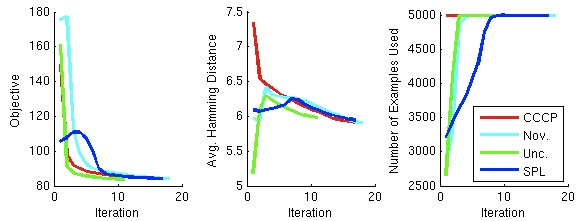
\includegraphics[scale = 0.7]{ExampleMotifRun_WithNovelty_small2.png}
\caption{Objective value, average hamming distance, and number of included training examples in each iteration for the four learning algorithms on a single protein, fold, and seed.}
\label{fig:exrun}
\end{figure}

The rightmost plot, which shows the number of examples used by the various algorithms over iterations, is very informative. The addition of examples is much more gradual in the SPL algorithm than in the SPL-Uncertainty or SPL-Novelty algorithms, not only in this particular run but in general. After just a couple of iterations, both the SPL-Uncertainty and SPL-Novelty algorithms had included all of the training examples. By examining the uncertainty, slack, and novelty values for the training examples over time, we identified the cause of this behavior: as better parameters are learned, the uncertainty and novelty drop much more quickly than the slack. In general, we note that because it adds all of the examples to the training set so quickly, the SPL-Uncertainty algorithm is more similar in its dynamics to CCCP than to SPL. For instance, the ``hump'' in the objective curve characteristic of standard SPL is absent from the objective curve of the SPL-Uncertainty algorithm. 

TODO: describe how 'dynamics are more similar to CCCP'.  Include results about annealing

As another measure of performance, we considered the Hamming distance (the minimum number of substitutions required to convert one string to another of equal length) between motifs in positive examples. The middle plot in Figure \ref{fig:exrun} shows the average Hamming distance for selected samples over iterations. Consistent with the observations in \cite{SPL}, we saw that the Hamming distance for SPL tended to start low, increase as more difficult examples are introduced, and then decrease again once all examples have been included. For SPL-Uncertainty, due to the rapid introduction of all examples, we see only a brief increase in average Hamming distance followed by a longer period of decrease. This observation supports the conclusion that, in general, SPL-Uncertainty is less of a departure from CCCP than SPL. 

TODO: Mention why hamming distance is lower to start for uncertainty: we include so few positive examples.  

%TODO **talk about annealing factor. what part of it is annealing factor and what part is order? We wondered whether the only difference was the same examples being added but faster for SPL-Uncertainty, so we plotted bla.

As a final area of investigation, we asked how different are the new criteria, uncertainty and novelty, from the original algorithm's criterion, slack? We wanted to understand whether uncertainty and novelty were adding examples in the same general order as slack-based SPL. To answer this question, we plotted the \emph{order} in which samples are first selected by one criterion against another, as shown in Figure \ref{fig:order}. A point at ($i$, $j$) indicates that the $i$-th example selected by criteria {\sc X} was the $j$-th point selected by criteria {\sc Y}.  If the criteria are equal the plot is a line, and if they are totally unrelated, the plot is white noise.  In SPL, examples are actually added in batches, so within a batch we ordered examples by increasing criterion value at time of addition.  In SPL an example may be included one iteration, then rejected in a later iteration, then included again.  In order to compare orderings across two different criteria, we included an example in the ordering at most once corresponding to the first SPL iteration in which it is included.  Finally, because there is only uncertainty over $\bf h$ in positive sequences, we only compare the order of inclusion of positive DNA sequences that bind to the protein.

\begin{figure}
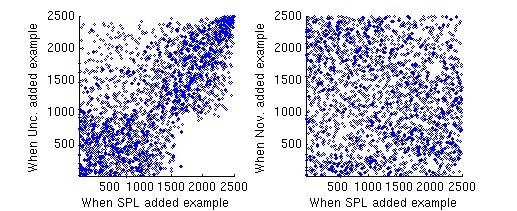
\includegraphics{ordercomp.png}
\caption{Comparison of order of inclusion of training examples for standard slack-based SPL and other selection criteria.  }
\label{fig:order}
\end{figure}

We first compare the best 2 selection criteria, slack and uncertainly, in the left-most plot.  We observe that they select from similar pools of points in the first and second halves of their training, as revealed by the two rectangular blocks in the bottom left and top right of the plot.  Interestingly, the points seem to be uniformly scattered within each rectangle.  This suggests that slack and uncertainty are somewhat similar, and helps understand how both algorithms do significantly better than {\sc CCCP} at avoiding really bad local optima.  Interestingly, both orderings agree most tightly on the very hardest samples, leading to a cluster in the top right of the graph.  This suggests that SPL may be more about excluding hard samples than choosing easy ones.

The right-most plot in Figure \ref{fig:order} shows that novelty and slack seem to be inversely related: higher densities of points in the top left and bottom right quadrants indicate that examples chosen early by slack are more likely to be chosen late by novelty, and vice versa. This is consistent with novelty getting stuck in really bad local optima significantly more often than slack.

(OUTLINE)
\begin{itemize}

\item Results were relatively similar and we were interested in understanding whether they were choosing the same examples. Show order comparison graph.
\item Show bounding box results. Wondering about non-maximal suppression. 
\end{itemize}

\begin{table}
\begin{center}
\subfigure[Final Objective Values] {
\begin{tabular}{|c|c|c|c|c|c|}
\hline Protein Number  & CCCP & SPL & Uncertainty & Novelty \\\hline
1 & \textbf{57.49} $\pm$ \textbf{1.70} & $57.80 \pm 1.47$ & $57.52 \pm 1.67$ & $95.01 \pm 45.06$\\
2 & $85.04 \pm 2.73$ & $84.67 \pm 3.14$ & \textbf{83.89} $\pm$ \textbf{2.26} & $84.08 \pm 1.14$\\
3 & $91.32 \pm 29.58$ & $78.27 \pm 4.51$ & \textbf{75.33} $\pm$ \textbf{4.27} & $105.63 \pm 36.40$\\
4 & $94.63 \pm 27.74$ & $79.93 \pm 1.59$ & \textbf{79.27} $\pm$ \textbf{1.06} & $80.45 \pm 2.81$\\
5 & $73.86 \pm 38.07$ & $54.26 \pm 1.09$ & \textbf{54.04} $\pm$ \textbf{0.84} & $111.90 \pm 46.77$ \\\hline
\end{tabular}
}
\subfigure[Train Errors (\%)] {
\begin{tabular}{|c|c|c|c|c|c|}
\hline Protein Number  & CCCP & SPL & Uncertainty & Novelty \\\hline
1 & $12.74 \pm 0.79$ & $12.79 \pm 0.75$ & \textbf{12.66} $\pm$ \textbf{0.74} & $27.76 \pm 18.17$\\
2 & $23.68 \pm 1.32$ & $23.07 \pm 1.27$ & \textbf{22.62} $\pm$ \textbf{0.90} & $23.01 \pm 0.33$\\
3 & $25.58 \pm 12.28$ & $19.90 \pm 1.76$ & \textbf{19.07} $\pm$ \textbf{1.65} & $31.49 \pm 15.14$\\
4 & $26.38 \pm 11.22$ & $21.30 \pm 1.57$ & ${20.46} \pm {0.58}$ & \textbf{20.33} $\pm$ \textbf{0.52}\\
5 & $20.27 \pm 14.88$ & $12.56 \pm 0.46$ & \textbf{12.49} $\pm$ \textbf{0.15} & $35.14 \pm 18.20$\\\hline
\end{tabular}
}
\subfigure[Test Errors (\%)] {
\begin{tabular}{|c|c|c|c|c|c|}
\hline Protein Number  & CCCP & SPL & Uncertainty & Novelty \\\hline
1 & \textbf{31.65} $\pm$ \textbf{0.43} & $31.77 \pm 0.47$ & \textbf{31.65}$\pm$ \textbf{0.35} & $39.03 \pm 8.96$\\
2 & $31.44 \pm 0.40$ & \textbf{30.83} $\pm$ \textbf{0.27} & $31.02 \pm 0.18$ & $31.44 \pm 0.36$\\
3 & $33.79 \pm 8.12$ & $30.33 \pm 0.77$ & \textbf{29.85} $\pm$ \textbf{0.51} & $37.99 \pm 9.82$\\
4 & $34.95 \pm 7.12$ & $31.49 \pm 0.30$ & \textbf{31.43} $\pm$ \textbf{0.43} & $31.38 \pm 0.58$\\
5 & $32.36 \pm 8.83$ & $27.97 \pm 0.27$ & \textbf{27.90} $\pm$ \textbf{0.28} & $41.22 \pm 10.76$\\\hline
\end{tabular}
}
\subfigure[Run Times (seconds)] {
\begin{tabular}{|c|c|c|c|c|c|}\hline
 CCCP & SPL & Uncertainty & Novelty \\\hline
$397.35 \pm 291.37$ & $642.61 \pm 330.48$ & $460.10 \pm 237.29$ & $3085.39 \pm 3151.12$\\\hline
\end{tabular}
}
\end{center}
\caption{The results (reported as mean $\pm$ standard deviation) for the four algorithms in the motif finding application. In general, the SPL-Uncertainty algorithm outperformed the other three and ran faster than the original SPL algorithm. }
\label{tbl:motif}
\end{table}


\section{Future Work}

There are several interesting directions for future investigation. Most immediately, the SPL-Uncertainty algorithm should be applied to other problems to determine whether its strong performance generalizes. We obtained preliminary results for the object localization problem described in \cite{SPL}. In this problem, the examples are images containing objects of a particular type (in our experiment, each image contained a certain type of mammal), and the goal is to determine which type of object each image contains. The hidden variable is the location of the bounding box surrounding the object. 

Our dataset, the same as that from \cite{SPL}, consisted of 271 images, each one containing one of 6 mammals. We used five folds (90\% train, 10\% test) to evaluate the algorithms and obtained the results displayed in Table \ref{tbl:bbox}.  


\begin{table}
\caption{The results (reported as mean $\pm$ standard deviation) for the three algorithms in the bounding box application. }
\begin{center}
\begin{tabular}{|c|c|c|c|}
\hline  & CCCP & SPL & Uncertainty \\\hline
Final Objective & $4.70 \pm 0.10$ & \textbf{4.42} $\pm$ \textbf{0.11} & $4.47 \pm 0.08$ \\\hline
Train Error (\%) & $0.33 \pm 0.16$ & \textbf{0.08} $\pm$ \textbf{0.16} & \textbf{0.08} $\pm$ \textbf{0.16}  \\ \hline
Test Error (\%) & $16.92 \pm 4.62$ & \textbf{16.15} $\pm$ \textbf{6.15} & \textbf{16.15} $\pm$ \textbf{6.16} \\ \hline
Run Time (sec) & $858.96 \pm 140.62$ & $1421.66 \pm 100.14$ & \textbf{544.32} $\pm$ \textbf{36.27} \\ \hline
\end{tabular}
\end{center}
\label{tbl:bbox}
\end{table}

we have several types of objects (in this case, different mammals) and 
 images containing a particular type of object .

bla.
\begin{itemize}
\item More principled manner of fitting the sigmoid to the 
\item Other applications
\item Wonder if novelty can be made faster -- a proxy that does not require solving a QP once per iteration per example. Caching results, etc.
\end{itemize}

\section{Conclusion}

We have explored 2 novel inclusion criteria for Self-Paced Learning ({\sc SPL}): \textbf{uncertainty} and \textbf{novelty}.  Of these, uncertainty performed better than slack in most cases, improving objective value and train/test error, and avoiding really bad local optima.  The performance of these two criteria are more similar to each other than to SPL on all metrics.  This supports the intuition that Self-Paced Learning works by learning a better hidden variable model, encoded in the parameters $\bf w$

Novelty, on the other hand, performed poorly compared to slack


TODO: annealing, some better some worse, show table.  Then we look at order.

TODO: entropy numbers aren't important, just the order and how they interact w/annealing.


(OUTLINE)
\begin{itemize}
\item Explain 
\end{itemize}

\section{Acknowledgments}

Ben and Pawan




\begin{thebibliography}{9}


\bibitem{SPL} P Kumar, B Packer, and D Koller. \emph{Self-Paced Learning for Latent Variable Models},
NIPS 2010. \url{http://ai.stanford.edu/~koller/Papers/Kumar+al:NIPS10.pdf}

\bibitem{SSVM} CN Yu, T Joachims. \emph{Learning Structural SVMs with Latent Variables}. \url{www.cs.cornell.edu/~cnyu/papers/icml09_latentssvm.pdf}

\bibitem{App1} PF Felzenszwalb, RB Girshick, D McAllester and D Ramanan. \emph{Object Detection with Discriminatively Trained
Part Based Models}.  \url{http://www.ics.uci.edu/~dramanan/papers/latentmix.pdf}

\bibitem{Mosek} The MOSEK Optimization Software. \url{http://www.mosek.com/}

\end{thebibliography}

\end{document}